%%%%%%%%%%%%%%%%%%%%%%%%%%%%%%%%%%%%%%%%%%%%%%%%%%%%%%%%%%%%%%%%%%%%%%%%%%%

\documentclass{standalone}

\usepackage{amsmath}
\usepackage{mathptmx}
\usepackage{pgfplots}
\usetikzlibrary{external}
\tikzexternalize{aluminium}
\pgfplotsset{compat=1.15}

%% IEEE uses Times Roman font, so we'll default to Times.
%% These three commands make up the entire times.sty package.
\renewcommand{\rmdefault}{ptm}
\renewcommand{\ttdefault}{pcr}
\normalfont\selectfont

\begin{document}

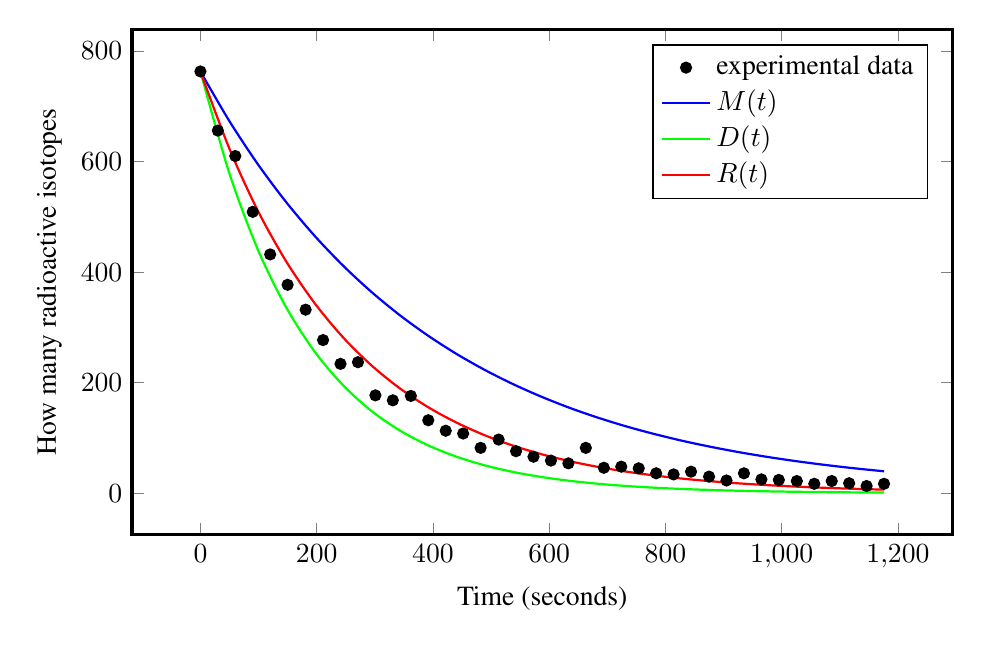
\begin{tikzpicture}
\tikzset{%%
  every mark/.append style={scale=1.0},%%
  scale=1.0%%
}
\pgfplotsset{%%
  every axis/.append style={font=\normalsize}%%
}
%%
\begin{axis}[%%
  axis line style=very thick,%%
  dotStyle/.style={mark size=2,black,mark color=black,mark=*,only marks},%%
  enlargelimits=true,%%
  height=8cm,%%
  legend cell align=left,%%
  legend pos=north east,%%
  plotStyle/.style={%%
    domain=0:1176,%%
    mark=none,%%
    smooth,%%
    thick%%
  },%%
  width=12cm,%%
  %% x axis
  xlabel={\normalsize Time~(seconds)},%%
  %% y axis
  ylabel={\normalsize How many radioactive isotopes},%%
  scaled y ticks=false,%%
  y tick label style=/pgf/number format/fixed%%
]
%%
%%
\addplot[dotStyle] coordinates {
  (0, 763)
  (30, 656)
  (60, 610)
  (90, 509)
  (120, 432)
  (150, 377)
  (181, 332)
  (211, 277)
  (241, 234)
  (271, 237)
  (301, 177)
  (331, 168)
  (362, 176)
  (392, 132)
  (422, 113)
  (452, 108)
  (482, 82)
  (513, 97)
  (543, 76)
  (573, 66)
  (603, 59)
  (633, 54)
  (663, 82)
  (694, 46)
  (724, 48)
  (754, 45)
  (784, 36)
  (814, 34)
  (844, 39)
  (875, 30)
  (905, 23)
  (935, 36)
  (965, 25)
  (995, 24)
  (1026, 22)
  (1056, 17)
  (1086, 22)
  (1116, 18)
  (1146, 13)
  (1176, 17)
};
\addlegendentry{experimental data}
%%
%%
%% The exponential model with mean decay factor.
\addplot+ [plotStyle,blue]
{763 * (0.927331^(x/30))};
\addlegendentry{$M(t)$}
%%
%%
%% The exponential model with decay rate of 1/6.
\addplot+ [plotStyle,green]
{763 * exp(-x/180)};
\addlegendentry{$D(t)$}
%%
%%
%% The exponential model with mean decay rate of r = 0.004058.
\addplot+ [plotStyle,red]
{763 * exp(-0.004058*x)};
\addlegendentry{$R(t)$}
\end{axis}
\end{tikzpicture}

\end{document}
